\begin{figure}[ht!]
    \centering
    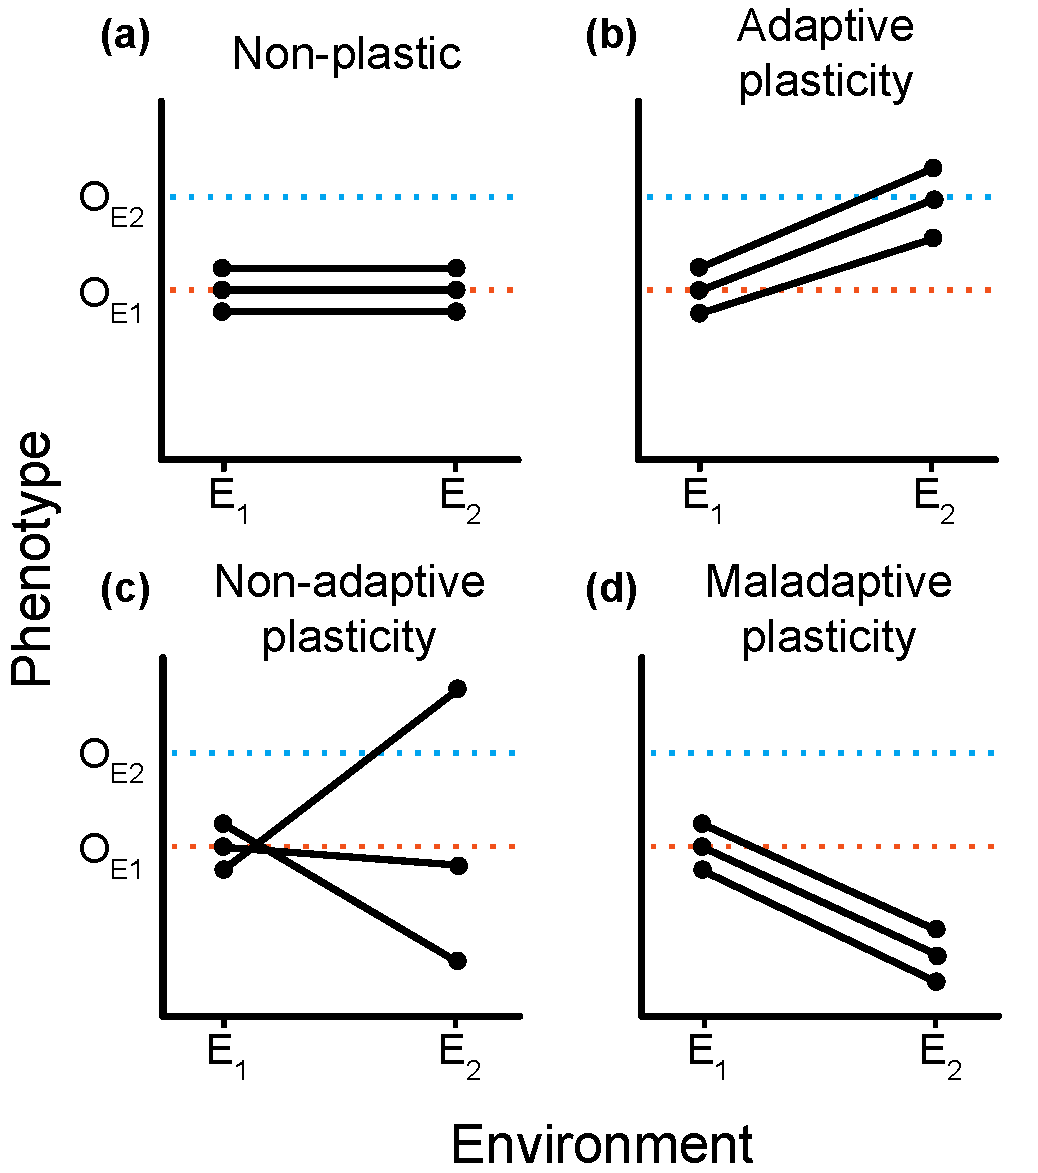
\includegraphics[width=0.65\textwidth]{media/reaction-norms.pdf}
    \caption{\small
    \textbf{Hypothetical reaction norms for genotypes that exhibit phenotypic variation.}
    In panels (a) through (d), two environments (denoted E$_1$ and E$_2$) are shown on the x-axis.
    The optimal phenotype in each of E$_1$ and E$_2$ (denoted O$_{\text{E}1}$ and O$_{\text{E}2}$, respectively) is shown on the y-axis.
    Each pair of points connected by a solid black line denotes a genotype, and the points represent the hypothetical phenotype expressed by organisms of that genotype within each environment.
    For each scenario, we overview our expectations for how populations would respond to a change from E$_1$ to E$_2$.
    (a) In non-plastic populations, we expect strong directional selection on mutations that move phenotypes toward O$_{\text{E}2}$ after the environment changes.
    (b) Adaptively plastic populations are already near the phenotypic optimum when the environment changes. As such, we would expect this population to remain relatively stable after the environment changes.
    (c) The population exhibits non-adaptive plasticity with substantial variation in how individuals respond to the environmental change. In this case, we expect plasticity to result in a rapid evolutionary response to the change in environment.
    (d) The population exhibits maladaptive plasticity relative to the given environmental change. When the environment changes, there is little variation for selection to act on, and without beneficial mutations, this population is at risk of extinction due to their maladaptive plastic response. 
    }
    \label{fig:reaction-norms}
\end{figure}

%%%%% OLD CAPTION

% (a) through (d) show four hypothetical reaction norm scenarios for two environments, E$_1$ (in red) to E$_2$ (in blue).  
% The optimal phenotypes for environments E$_1$ and E$_2$ are different (O$_{\text{E}1}$ and O$_{\text{E}2}$, respectively).
% In each of the four reaction norm scenarios, populations are well-adapted to E$_1$.
% In (a), genotypes in the population are non-plastic, and as such, we would expect strong directional selection on mutations that move phenotypes toward O$_{\text{E}2}$ after the environment changes.
% In (b), genotypes in the population are adaptively plastic. 
% That is, phenotypic changes induced by the environment change to E$_2$ are already near the optimum, and as such, we would expect this population to remain relatively stable after the environment changes.
% In (c), the population exhibits non-adaptive plasticity with substantial variation in how individuals respond to the environmental change. 
% In this case, we expect plasticity to result in a rapid evolutionary response to the change in environment.  
% In (d), the population exhibits maladaptive plasticity relative to the given environmental change. 
% When the environment changes, there is little variation for selection to act on, and without beneficial mutations, this population may be at risk of extinction due to their maladaptive plastic response.